% translate_docs: ./cars/E-GMP_gen1/Ioniq5/selectable_CAN_Ioniq5_install.tex @ 70713bdb023d4770e12e70b4f55f50b0d8b74a46
\documentclass[superscriptaddress,onecolumn,floatfix]{revtex4-2}

\usepackage{graphicx}
\usepackage{epsfig}
\usepackage{color}
\usepackage{amssymb}
\usepackage{amsmath}
\usepackage{array}
\usepackage[loose]{units}
\usepackage{hyperref}
\usepackage{cleveref}
\usepackage{braket}
\usepackage[caption=false]{subfig}
\usepackage[german]{babel}
\usepackage{letltxmacro}

\pdfcompresslevel=9

\LetLtxMacro{\ORIGselectlanguage}{\selectlanguage}
\makeatletter
\DeclareRobustCommand{\selectlanguage}[1]{%
    \@ifundefined{alias@\string#1}
      {\ORIGselectlanguage{#1}}
      {\begingroup\edef\x{\endgroup
         \noexpand\ORIGselectlanguage{\@nameuse{alias@#1}}}\x}%
}
\newcommand{\definelanguagealias}[2]{%
  \@namedef{alias@#1}{#2}%
}
\makeatother

\definelanguagealias{de}{german}


\begin{document}
\selectlanguage{de}

\begin{abstract}
  Diese Anleitung führt Sie durch die notwendigen Schritte zur Installation des wählbaren CAN-Kabelbaums in Ihrem Ioniq 5 (Modelljahre 2021–2024). Siehe auch \href{https://youtube.com/playlist?list=PLYCTmVJH4UYqnw87UZAaqMo1GrOv0cJaL}{Videoanleitungen}:
  \begin{description}
    \item[Schritt 1: 12V-Anschluss trennen] \href{https://youtu.be/ePBdyeBYKk4}{Videoanleitung}
    \item[Schritt 2: Kabelbaum installieren] \href{https://youtu.be/kVvkR4ZLFMI}{Montageanleitung für den Gurt}
  \end{description}
\end{abstract}
\title{Auswählbarer CAN-Installationsleitfaden}
\author{Electroniq Buttons Boutique}
\email{support@electroniqbuttons.com}
% \affiliation{\GOE}
% \author{Benjamin J. McMorran}
% \email{mcmorran@uoregon.edu}
% \affiliation{\UO}
\date{\today}

\maketitle

% \begin{figure}[h]
%   \subfloat[]{\label{subfig:overview:harness}
%   \includegraphics[height=1.95in]{../../../harnesses/head_unit_MITM/photos/whole_harness.jpg} } \\
%   \subfloat[]{\label{subfig:overview:trim}
%   \includegraphics[width=6in]{photos/overview_labeled.jpg} }
%    \caption{(a) Man-in-the-middle harness. (b) Overview of trim panels involved. \label{fig:overview}}
% \end{figure}

\section{Einführung}
Diese Anleitung beschreibt die Schritte zum Einbau des auswählbaren CAN-Kabelbaums in ein Ioniq 5 ICU. Siehe auch \href{https://github.com/dragz/explorationsincarhacking/blob/main/articles/getting_past_the_secure_gateway/getting_past_the_secure_gateway.md}{diese Anweisungen} zur Identifizierung und zum Zugriff auf den ICU-H-Anschluss.

Erforderliche Werkzeuge:
\begin{enumerate}
  \item 10-mm-Steckschlüssel oder verstellbarer Schraubenschlüssel für 12-V-Batterie
  \item Schere
\end{enumerate}

Kit-Bestandteile:
\begin{enumerate}
  \item Wählbarer CAN-Kabelbaum
  \item WiCAN
  \item 60-mm-OBD-Halterung
  \item 70 mm doppelseitiges Klebeband (zwei Stücke zur Sicherheit enthalten)
  \item 4 Kabelbinder
\end{enumerate}

\section{Schritt 1: Den Minuspol der 12-V-Batterie abklemmen.} \label{sect:0}
Trennen Sie immer zuerst die 12-V-Batterie, bevor Sie irgendwelche elektrischen Steckverbinder entfernen! Das Entfernen eines stromführenden Steckers kann eine Entladung verursachen und einen Stecker oder das Steuergerät Ihres Autos zerstören.

Schritt-für-Schritt-Anleitung:
\begin{enumerate}
  \item Motorhaube öffnen (Abbildung \ref{subfig:12V:hood})
  \item Öffnen Sie den Frunk. 
  \item Entfernen Sie die Abdeckung für die 12-V-V-Schnittstelle (Abbildung \ref{subfig:12V:panel})
  \item Die Mutter auf der Minusseite mit einer 10-mm-Nuss lösen (Abbildung \ref{subfig:12V:nut})
  \item Entfernen Sie den Minuspol (Abbildung \ref{subfig:12V:terminal})
\end{enumerate}

\begin{figure}[h]
  \subfloat[]{\label{subfig:12V:hood}
  \includegraphics[height=1.5in]{photos/open_hood.jpg} } 
  \subfloat[]{\label{subfig:12V:panel}
  \includegraphics[height=1.5in]{photos/remove_panel.jpg} }  \\
  \subfloat[]{\label{subfig:12V:nut}
  \includegraphics[height=1.5in]{photos/loosen_nut.jpg} } 
  \subfloat[]{\label{subfig:12V:terminal}
  \includegraphics[height=1.5in]{photos/disconnect_terminal.jpg} } 
   \caption{(a) Öffnen Sie die Motorhaube. (b) Entfernen Sie die Abdeckung des 12-V-Anschlusses. (c) Lösen Sie die Mutter am Minuspol. (d) Entfernen Sie den Minuspol. \label{fig:12V}}
\end{figure}

\section{Schritt 2: Kabelbauminstallation} \label{sect:2}
Dieser Schritt umfasst den Einbau des Kabelbaums in die Intensivstation. 

Schritt-für-Schritt-Anleitung:
\begin{enumerate}
  \item (Optional) Entfernen Sie ICU-H nach \href{https://github.com/dragz/explorationsincarhacking/blob/main/articles/getting_past_the_secure_gateway/getting_past_the_secure_gateway.md}{diese Anweisungen}
  \item Installieren Sie den Sicherungsabgriff in den freien Steckplatz 2 für Dauerbetrieb oder in den freien Steckplatz 1 für Betrieb bei eingeschaltetem Fahrzeug (Abbildung \ref{subfig:harness:fusetap})
  \item ICU-H-Anschluss entfernen (Abbildung \ref{subfig:harness:ICU-H})
  \item Führen Sie die weibliche Seite des Gurtes in die Intensivstation ein. 
  \item Stecken Sie den zuvor entfernten weiblichen Stecker in die männliche Seite des Kabelbaums. 
  \item Montieren Sie die Halterung an der Seite des blauen Steckers, so dass die OBD-Seite nach unten zeigt (Abbildung). \ref{subfig:harness:obd_mount})
  \item Setzen Sie den OBD-Anschluss in die Halterung ein.
  \item Stecken Sie WiCAN in den OBD-Anschluss.
\end{enumerate}

\begin{figure}[h]
  \subfloat[]{\label{subfig:harness:fusetap}
  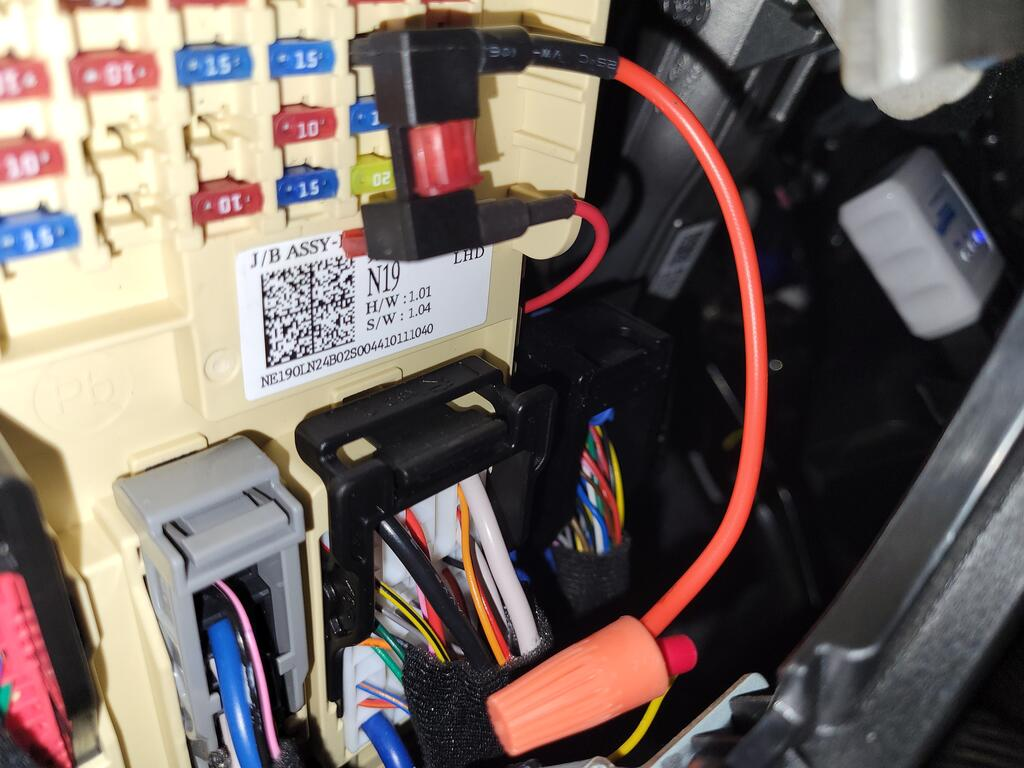
\includegraphics[height=1.5in,angle=0]{photos/fuse_tap_in_wrong.jpg} } 
  \subfloat[]{\label{subfig:harness:ICU-H}
  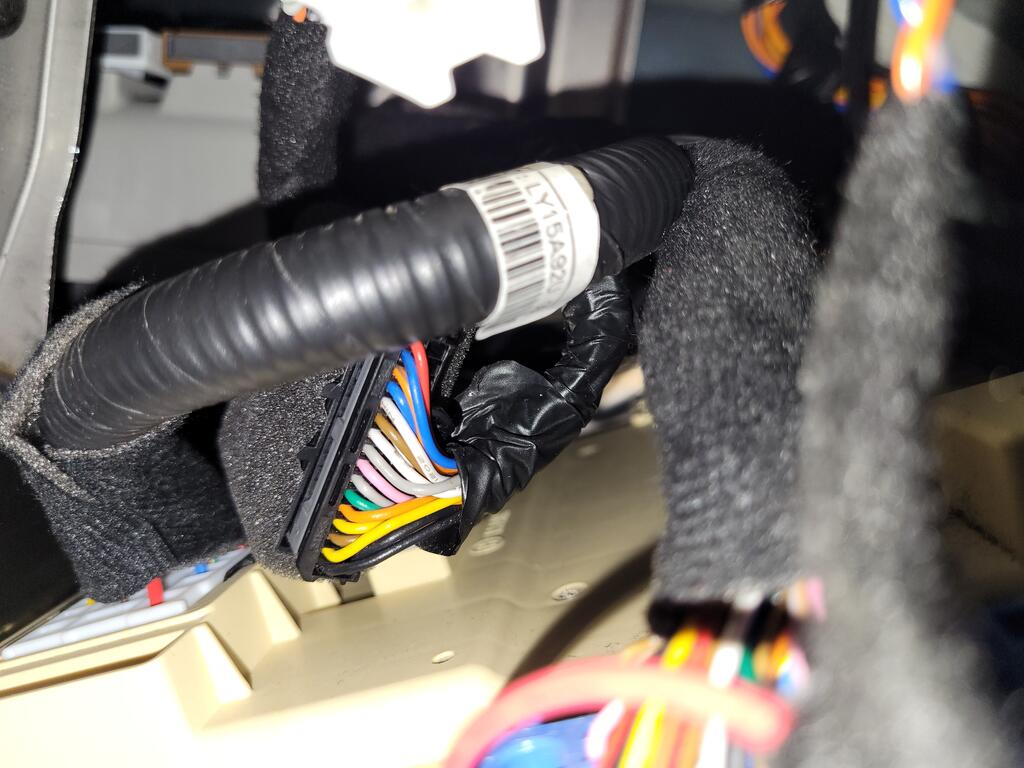
\includegraphics[height=1.5in,angle=0]{photos/icu-h_harness_in.jpg} }  
  \subfloat[]{\label{subfig:harness:obd_mount}
  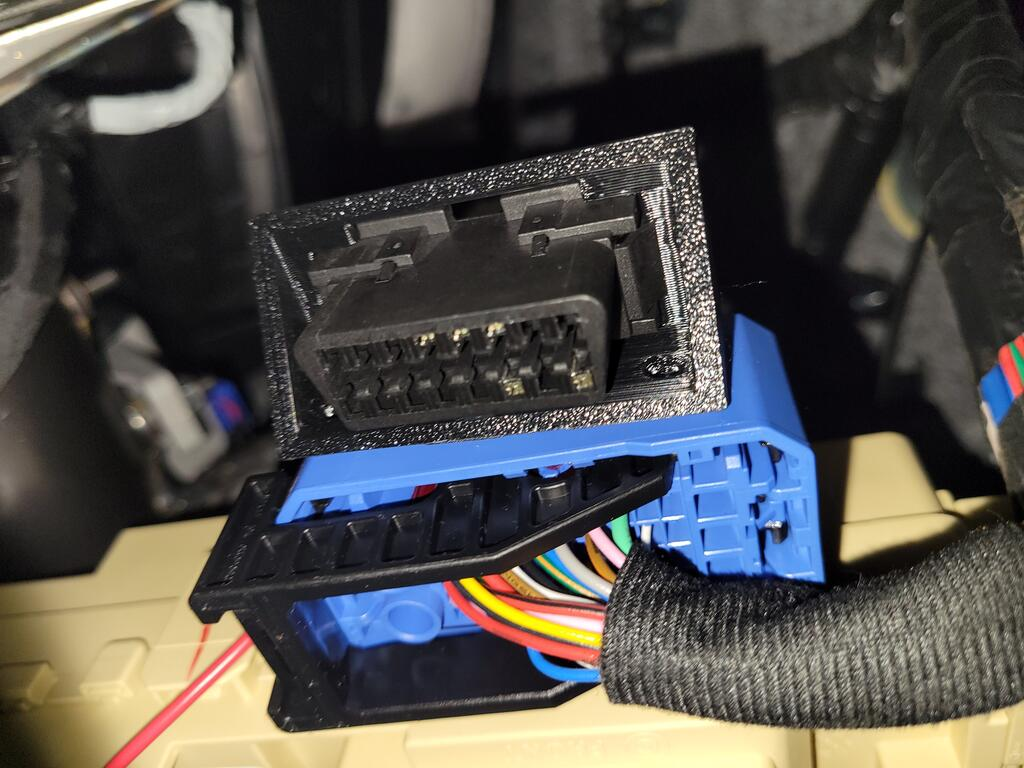
\includegraphics[height=1.5in,angle=0]{photos/obd_mounted_icuh.jpg} } 
   \caption{(a) Der Sicherungsabgriff für die Dashcam ist an Reserve 2 angeschlossen. Beachten Sie, dass dies wie abgebildet nicht funktioniert und eine zweite Sicherung am unteren Sicherungsabgriff erfordert. (b) ICU-H (grüner Pfeil) mit installiertem Kabelbaum; der Stecker des Kabelbaums (roter Pfeil) ist mit dem originalen weiblichen Stecker verbunden. (c) Die OBD-Buchse ist an der Halterung montiert. \label{fig:harness}}
\end{figure}

\section{Schritt 3: Aufräumen} \label{sect:4}
Schließen Sie den Minuspol der 12-V-Batterie wieder an. Das WiCAN-Display sollte sofort blau leuchten. \href{https://meatpihq.github.io/wican-fw/config/wifi}{Ändern Sie Ihr WiCAN-Passwort!}Sie können Ihr WiCAN-Gerät direkt verbinden, indem Sie ein WLAN-Netzwerk mit dem Namen „WiCAN“ suchen.\_xxxxxxx' und geht zu \href{http://192.168.80.1/}{http://192.168.80.1/} in Ihrem Browser.
\appendix 
\bibliographystyle{apsrev4-1}
\bibliography{stemh_model}{}
\end{document}
